\documentclass[conference]{IEEEtran}
\IEEEoverridecommandlockouts
\usepackage{cite}
\usepackage{amsmath,amssymb,amsfonts}
\usepackage{algorithmic}
\usepackage{graphicx}
\graphicspath{{./}{../docs/}{docs/}}
\usepackage{textcomp}
\usepackage{xcolor}
\usepackage{booktabs}
\usepackage{bm}
\usepackage{url}

\def\BibTeX{{\rm B\kern-.05em{\sc i\kern-.025em b}\kern-.08em
    T\kern-.1667em\lower.7ex\hbox{E}\kern-.125emX}}

\begin{document}

\title{Mitigating Catastrophic Forgetting and Exploitability in Competitive Multi-Agent Reinforcement Learning via Dual-Archive Co-Evolution}

\author{
\IEEEauthorblockN{Navadeep G.}
\IEEEauthorblockA{\textit{Department of Mathematics} \\
\textit{SVNIT Surat}, India \\
nindra.navadeep11@gmail.com}
\and
\IEEEauthorblockN{Brij Radadiya}
\IEEEauthorblockA{\textit{Department of Mathematics} \\
\textit{SVNIT Surat}, India \\
radadiyabrij43@gmail.com}
\and
\IEEEauthorblockN{Shrey Marakana}
\IEEEauthorblockA{\textit{Department of Mathematics} \\
\textit{SVNIT Surat}, India \\
marakanashrey2426@gmail.com}
\and
\IEEEauthorblockN{Shree Pastagia}
\IEEEauthorblockA{\textit{Department of Mathematics} \\
\textit{SVNIT Surat}, India \\
shreepastagia126219@gmail.com}
}

\maketitle

\begin{abstract}
In competitive multi-agent reinforcement learning (MARL), unanchored self-play frequently degenerates into cyclic non-stationarity—the classic Red Queen effect—and catastrophic forgetting, wherein policies overfit to transient opponent behaviors while discarding previously mastered competencies. This paper investigates these pathologies within the Three Bridges Arena, an asymmetric zero-sum spatial gridworld that instantiates an irreducible Rock-Paper-Scissors dilemma where defensive pure strategies cannot simultaneously protect all transit bottlenecks. We propose a symmetric Dual-Archive Co-Evolutionary architecture combined with zero-sum discounted potential-based reward shaping that mathematically guarantees optimal policy invariance under discount factor $\gamma = 0.99$ in accordance with Ng et al. (1999). Through standardized empirical game-theoretic analysis (EGTA) across 150 paired evaluation seeds, we demonstrate that naive self-play suffers severe route collapse (46.0\% North vs. 16.1\% South bridge traversal, with 17.3\% unforced navigation timeouts) and elevated exploitability ($\delta = 0.160$). In contrast, Dual-Archive co-evolution preserves balanced multi-corridor exploratory competence, achieving an empirical Shannon route entropy of 1.567 bits (98.9\% of the theoretical maximum of 1.585 bits) with 0.0\% timeouts. Furthermore, the dual historical reservoir reduces minimax exploitability to $\delta = 0.140$ and elevates the worst-case security level from $-0.207$ to $-0.187$. While raw pooled win rates between methods remain statistically indistinguishable ($\Delta = -0.6\%$, $p = 0.771$), these results illustrate that raw win rates are fundamentally deceptive in non-stationary MARL, whereas route entropy and empirical minimax exploitability isolate genuine strategic robustness.
\end{abstract}

\begin{IEEEkeywords}
Multi-Agent Reinforcement Learning, Self-Play, Catastrophic Forgetting, Nash Equilibrium, Empirical Game-Theoretic Analysis, Potential-Based Reward Shaping, Zero-Sum Games.
\end{IEEEkeywords}

\section{Introduction}
Competitive Multi-Agent Reinforcement Learning (MARL) has driven major breakthroughs across complex game domains, including chess, Go, poker, and real-time strategy environments \cite{silver2016mastering, vinyals2019alphastar, berner2019dota}. In these settings, self-play serves as an automated curriculum: agents discover counter-strategies by competing against concurrently learning copies of themselves.

Despite empirical successes, unanchored self-play exhibits well-known game-theoretic vulnerabilities \cite{balduzzi2019open}. Because both agents update their parameters simultaneously, the optimization landscape is non-stationary from the perspective of either learner. This non-stationarity frequently triggers the evolutionary dynamic known as the \textit{Red Queen Effect} \cite{cliff1995tracking}: agents must continuously adapt simply to maintain relative performance parity. In games characterized by intransitive strategy structures (e.g., spatial variants of Rock-Paper-Scissors), independent gradient descent typically induces closed behavioral cycling rather than monotonic convergence toward a minimax optimal Nash equilibrium.

Closely coupled with policy cycling is the pathology of \textit{catastrophic forgetting} \cite{mccloskey1989catastrophic}. When an opponent shifts defensive focus from Route A to Route B, policy gradients penalize Route A and incentivize Route B. Consequently, gradient updates alter neural network representations to specialize against the immediate adversary, overwriting policy weights that successfully traversed Route A. When the opponent subsequently shifts back to Route B, the agent is re-exploited, causing persistent cyclic forgetting.

To systematically analyze and resolve this problem, this paper examines the \textit{Three Bridges Arena}, a discrete two-player zero-sum Markov gridworld designed around an asymmetric spatial bottleneck. An Attacker agent navigates across a river partitioned by four impassable obstacles and three bridge choke points (North, Center, South) to capture a fortified Citadel, while a Defender agent maneuvers to intercept the Attacker. Because the Defender occupies only a single grid cell and moves at speed parity, no deterministic pure strategy can simultaneously guard all three apertures.

To overcome policy cycling and catastrophic forgetting in this setting, we make the following contributions:
\begin{enumerate}
    \item \textbf{Mathematical Formulation and Invariant Guarantee:} We formalize the spatial bottleneck interaction as a finite zero-sum Markov game. We integrate discounted potential-based reward shaping with both target-advance and pursuit-evasion components, preserving the strict zero-sum invariant ($R_A + R_D \equiv 0.000000$) while guaranteeing invariance of the Nash equilibrium under discount factor $\gamma = 0.99$ (Ng et al. \cite{ng1999policy}; Devlin and Kudenko \cite{devlin2011theoretical}).
    \item \textbf{Dual-Archive Co-Evolutionary Framework:} We implement a symmetric multi-agent architecture maintaining persistent historical snapshot reservoirs for both Attacker and Defender. Policies train on a tripartite mixture of active self-play (60\%), active Attacker vs. archived Defender (20\%), and archived Attacker vs. active Defender (20\%).
    \item \textbf{Shannon Route Entropy Metric for Spatial Forgetting:} We establish an information-theoretic metric measuring the deviation of empirical river crossings from the theoretical maximum mixed strategy entropy ($H_{\max} = \log_2(3) \approx 1.585$ bits).
    \item \textbf{Empirical Game-Theoretic Analysis (EGTA):} We construct a spatial meta-game payoff matrix against an archetypal adversary suite, computing empirical minimax game values, security levels ($v_{\text{sec}}$), and exploitability distances ($\delta$).
    \item \textbf{Empirical Validation:} Across 150 standardized paired evaluation seeds, we show that Dual-Archive co-evolution prevents catastrophic route collapse (achieving $1.567$ bits, $98.9\%$ of theoretical maximum entropy) with 0.0\% timeouts, while reducing empirical exploitability from $\delta = 0.160$ to $0.140$ and raising the worst-case security floor from $-0.207$ to $-0.187$.
\end{enumerate}

\section{Related Work}

\subsection{Self-Play and Policy Cycling in MARL}
Self-play training traces back to TD-Gammon \cite{tesauro1995temporal} and has been central to modern multi-agent milestones \cite{silver2016mastering, vinyals2019alphastar, berner2019dota}. However, theoretical analysis shows that independent gradient ascent in multi-agent systems often diverges or enters limit cycles in games with intransitive dynamics \cite{balduzzi2019open}. Cliff and Miller \cite{cliff1995tracking} characterized this phenomenon in co-evolutionary algorithms as the Red Queen dynamic. Without memory or population diversity, agents continuously chase moving targets without making genuine global progress.

\subsection{Memory Reservoirs, Double Oracle, and PSRO}
Game theory addresses policy cycling through Fictitious Play \cite{brown1951iterative}, in which players best-respond to the empirical average strategy of their opponent's historical actions. In high-dimensional policy spaces, the Double Oracle algorithm \cite{mcmahan2003planning} iteratively computes minimax equilibria over restricted strategy sets. Lanctot et al. \cite{lanctot2017unified} generalized this concept to deep reinforcement learning via Policy-Space Response Oracles (PSRO), where reinforcement learning oracles generate best responses against mixed meta-strategies. Neural Fictitious Self-Play (NFSP) \cite{heinrich2016deep} similarly utilizes transition replay buffers to approximate fictitious play in extensive-form games. 

While landmark architectures such as AlphaStar \cite{vinyals2019alphastar} deploy vast, asymmetrical league-training frameworks involving main agents and specialized exploiter agents, such setups require prohibitive compute infrastructure. Our Dual-Archive framework introduces a symmetrical, lightweight snapshot reservoir specifically tailored for two-player zero-sum spatial interactions.

\subsection{Potential-Based Reward Shaping in Zero-Sum Games}
Reward sparsity is an acute challenge in multi-agent navigation. Potential-Based Reward Shaping (PBRS), introduced by Ng et al. \cite{ng1999policy}, guarantees that adding a difference of potentials $F(s, s') = \gamma \Phi(s') - \Phi(s)$ preserves the set of optimal policies in single-agent Markov Decision Processes. Devlin and Kudenko \cite{devlin2011theoretical} extended PBRS to multi-agent stochastic games, showing that if shaping is applied symmetrically such that $\sum_{i} F_i(s, s') = 0$, the zero-sum structural invariant is preserved and the underlying Nash equilibria remain intact.

\section{Game Formulation and Theoretical Framework}

\subsection{Two-Player Zero-Sum Markov Game Formalism}
We formulate the competitive spatial interaction as a discrete-time, two-player zero-sum Markov game defined by the tuple:
\begin{equation}
\mathcal{M} = \langle \mathcal{S}, \mathcal{A}_1, \mathcal{A}_2, \mathcal{P}, \mathcal{R}_1, \mathcal{R}_2, \gamma \rangle
\end{equation}
where:
\begin{itemize}
    \item $\mathcal{S} \subset [0, 1]^6$ is the continuous normalized observation space representing the spatial coordinates of both agents and the objective target.
    \item $\mathcal{A}_1, \mathcal{A}_2$ are discrete action spaces for Player 1 (Attacker) and Player 2 (Defender), each of cardinality $|\mathcal{A}_i| = 5$.
    \item $\mathcal{P}: \mathcal{S} \times \mathcal{A}_1 \times \mathcal{A}_2 \to \Delta(\mathcal{S})$ denotes the deterministic state transition probability distribution governed by the grid dynamics.
    \item $\mathcal{R}_1, \mathcal{R}_2: \mathcal{S} \times \mathcal{A}_1 \times \mathcal{A}_2 \to \mathbb{R}$ are the scalar reward functions satisfying the strict zero-sum condition $\mathcal{R}_1(s, a_1, a_2) + \mathcal{R}_2(s, a_1, a_2) = 0, \forall s, a_1, a_2$.
    \item $\gamma \in [0, 1)$ is the temporal discount factor, set to $\gamma = 0.99$.
\end{itemize}

\subsection{Spatial Topology: The Three Bridges Arena}
The game is instantiated on a 2D discrete coordinate lattice of dimensions $W = 11$ ($X \in \{0, \dots, 10\}$) and $H = 7$ ($Y \in \{0, \dots, 6\}$). The arena is partitioned longitudinally by a river barrier located at column $X = 5$:
\begin{itemize}
    \item \textbf{Infiltration Basin ($X \in [0, 4]$):} The Attacker spawns uniformly across coordinates $X_A \in [0, 3], Y_A \in [0, 6]$.
    \item \textbf{River Barrier ($X = 5$):} The column contains four impassable terrain pillars at $(5, 0), (5, 2), (5, 4), (5, 6)$ and three passable bridge apertures:
    \begin{align}
    \text{North Bridge:} \quad & b_N = (5, 1) \\
    \text{Center Bridge:} \quad & b_C = (5, 3) \\
    \text{South Bridge:} \quad & b_S = (5, 5)
    \end{align}
    \item \textbf{Defensive Basin ($X \in [6, 10]$):} The Defender spawns uniformly across coordinates $X_D \in [6, 9], Y_D \in [0, 6]$ (excluding the Citadel cell).
    \item \textbf{Citadel Target:} A static terminal capture objective located at $(X_T, Y_T) = (10, 3)$.
\end{itemize}

\subsection{State Representation and Action Dynamics}
The global state observation $s_t \in \mathcal{S}$ is normalized over coordinate dimensions $(W-1)$ and $(H-1)$:
\begin{equation}
s_t = \left[ \frac{x_A}{10}, \frac{y_A}{6}, \frac{x_D}{10}, \frac{y_D}{6}, \frac{x_T}{10}, \frac{y_T}{6} \right]^T
\end{equation}
Normalizing by maximal indices guarantees $s_t \in [0, 1]^6$, stabilizing neural value baseline updates.

At each discrete time step $t$, agents execute actions simultaneously from the discrete set $\mathcal{A} = \{\text{UP}, \text{DOWN}, \text{LEFT}, \text{RIGHT}, \text{STAY}\}$. Transitions obey:
\begin{equation}
\bm{p}_{i, t+1} = \bm{p}_{i, t} + \bm{v}(a_{i, t})
\end{equation}
subject to boundary constraints $0 \le x < 11$, $0 \le y < 7$, and obstacle exclusion $(x, y) \notin \{(5, 0), (5, 2), (5, 4), (5, 6)\}$. Attempts to breach boundary walls or impassable pillars result in zero displacement ($\bm{p}_{i, t+1} = \bm{p}_{i, t}$).

\subsection{Terminal Conditions and Mutual Priority}
An episode terminates immediately upon the occurrence of any of the following mutually exclusive conditions:
\begin{enumerate}
    \item \textbf{Citadel Infiltration:} The Attacker occupies the Citadel cell ($\bm{p}_A = (10, 3)$). The terminal payoffs are $R_A = +10, R_D = -10$.
    \item \textbf{Interception / Capture:} The Defender intercepts the Attacker prior to Citadel entry. Interception occurs if $\bm{p}_{A, t+1} = \bm{p}_{D, t+1}$ (co-location) or $\bm{p}_{A, t+1} = \bm{p}_{D, t} \land \bm{p}_{D, t+1} = \bm{p}_{A, t}$ (crossing-swap capture). The terminal payoffs are $R_A = -10, R_D = +10$.
    \item \textbf{Horizon Truncation:} Elapsed time steps reach $T_{\max} = 75$ without Citadel reach or interception. The terminal payoffs are $R_A = 0, R_D = 0$.
\end{enumerate}
Terminal priority is strictly enforced: if the Attacker reaches $(10, 3)$ simultaneously with Defender interception, Citadel capture takes absolute priority ($\text{caught} = \text{raw\_caught} \land \neg \text{reached\_target}$), eliminating ambiguous dual-win credit assignment.

\subsection{The Spatial Rock-Paper-Scissors Dilemma}
The Three Bridges topology establishes an intractable pure-strategy dilemma. Let $S_A = \{b_N, b_C, b_S\}$ and $S_D = \{g_N, g_C, g_S\}$ denote the abstract pure route choices for Attacker traversal and Defender bottleneck guarding. The Defender has speed parity with the Attacker ($1 \text{ cell/step}$) and occupies exactly one coordinate. The Manhattan transit distance between outer bridges $b_N$ and $b_S$ is 4 steps, whereas an Attacker at the river barrier can transit across the river in a single forward step. Consequently:
\begin{equation}
\forall s_D \in S_D, \quad \exists s_A \in S_A \quad \text{s.t.} \quad \mathcal{P}(\text{breach} \mid s_A, s_D) = 1.0
\end{equation}
If the Defender commits to guarding $b_N$, the Attacker exploits $b_S$. If the Defender moves to $b_S$, the Attacker shifts to $b_C$ or $b_N$.

\textbf{Theorem 1 (Non-Existence of Pure Strategy Equilibrium):} \textit{In the simplified static Three Bridges bottleneck matrix game, there exists no pure strategy Nash equilibrium. The unique minimax Nash equilibrium is the uniform mixed strategy where both players select each bridge with probability $p^* = \frac{1}{3}$.}

\textit{Proof Sketch:} Consider the $3 \times 3$ zero-sum matching game where the Defender successfully intercepts if choosing the identical bridge, earning payoff $+1$, while the Attacker breaches if choosing an unguarded bridge, earning payoff $-1$ for the Defender. The payoff matrix $M_D$ for the Defender is:
\begin{equation}
M_D = \begin{bmatrix} +1 & -1 & -1 \\ -1 & +1 & -1 \\ -1 & -1 & +1 \end{bmatrix}
\end{equation}
For any pure strategy $e_i$, $\min_j (e_i^T M_D)_j = -1$. For the uniform mixed strategy $\bm{q}^* = [\frac{1}{3}, \frac{1}{3}, \frac{1}{3}]^T$, the expected payoff against any pure Attacker action $j$ is $\bm{q}^{*T} M_D e_j = \frac{1}{3}(+1) + \frac{2}{3}(-1) = -\frac{1}{3}$. By the Minimax Theorem \cite{von1944theory}, the value of the game is $v^* = -\frac{1}{3}$, uniquely satisfied by $\bm{p}^* = \bm{q}^* = [\frac{1}{3}, \frac{1}{3}, \frac{1}{3}]^T$. \hfill $\blacksquare$

\subsection{Zero-Sum Discounted Potential-Based Reward Shaping}
Because sparse terminal rewards ($\pm 10$ at $t \le 75$) induce high policy variance and sluggish early exploration, we integrate continuous potential-based reward shaping.

The target distance potential $D_A(x, y)$ is defined piecewise across the river:
\begin{equation}
D_A(x, y) = \begin{cases} 
\min_{b_y \in \{1, 3, 5\}} \left( |x - 4| + |y - b_y| + 6 + |b_y - 3| \right), & x \le 4 \\
|x - 10| + |y - 3|, & x > 4
\end{cases}
\end{equation}
The additional term $|b_y - 3|$ accounts for the vertical distance from each bridge exit to the Citadel centerline ($y=3$), ensuring exact step-wise distance monotonicity across all three bridge corridors. Under discount factor $\gamma = 0.99$, the target-advance shaping component is:
\begin{equation}
F_{\text{tgt}}(s, s') = \alpha_{\text{tgt}} \left[ D_A(s) - \gamma D_A(s') \right]
\label{eq:shaping_tgt}
\end{equation}
where $\alpha_{\text{tgt}} = 0.3$.

To balance offensive progression with tactical interception, we include a relative pursuit-evasion shaping potential $D_{\text{rel}}(s) = |x_A - x_D| + |y_A - y_D|$ with scaling factor $\alpha_{\text{rel}} = 0.2$:
\begin{equation}
F_{\text{rel}}(s, s') = \alpha_{\text{rel}} \left[ D_{\text{rel}}(s) - \gamma D_{\text{rel}}(s') \right]
\label{eq:shaping_rel}
\end{equation}
The joint shaping rewards for Attacker and Defender are formulated symmetrically:
\begin{align}
F_A(s, s') &= +F_{\text{tgt}}(s, s') - F_{\text{rel}}(s, s') \\
F_D(s, s') &= -F_{\text{tgt}}(s, s') + F_{\text{rel}}(s, s')
\end{align}
Because $F_A(s, s') + F_D(s, s') \equiv 0.000000$ identically at every transition, total reward satisfies:
\begin{equation}
R_A(s, a_1, a_2) + R_D(s, a_1, a_2) \equiv 0.000000, \quad \forall s, s' \in \mathcal{S}
\end{equation}
By Devlin and Kudenko \cite{devlin2011theoretical}, symmetric potential shaping does not alter the Nash equilibrium strategy set of the underlying stochastic game.

\begin{figure}[t]
\centering
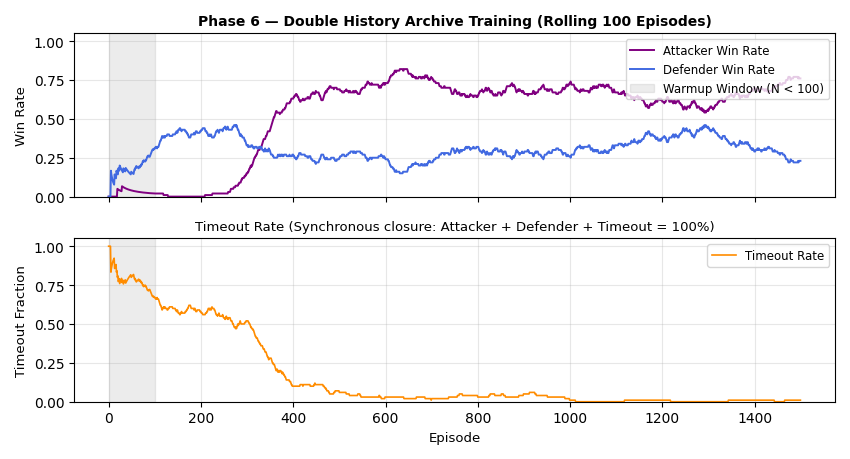
\includegraphics[width=0.92\columnwidth]{phase6_archive_curve.png}
\caption{Dual-Archive training dynamics across 1,500 episodes. Top: Rolling win rates for Attacker (purple, stabilizing near $\approx 65\%$) and Defender (blue, stabilizing near $\approx 33\%$), reflecting the inherent structural advantage of 3 bridges against 1 defender. Bottom: Decline in episode timeout rate from $\approx 80\%$ during initial exploration to below 2\% at convergence.}
\label{fig:training_curve}
\end{figure}

\section{Dual-Archive Co-Evolutionary Framework}

\subsection{The Vulnerability of Unanchored Self-Play}
In standard self-play (Phase 4), parameter vectors $\theta_A$ and $\theta_D$ are optimized directly against each other:
\begin{align}
\theta_{A, k+1} &\leftarrow \theta_{A, k} + \eta_A \nabla_{\theta_A} \mathcal{J}_A(\theta_{A, k}, \theta_{D, k}) \\
\theta_{D, k+1} &\leftarrow \theta_{D, k} + \eta_D \nabla_{\theta_D} \mathcal{J}_D(\theta_{A, k}, \theta_{D, k})
\end{align}
Because gradient updates occur concurrently, neither policy provides a stationary distribution. When $\theta_{A}$ learns to breach the North bridge, $\theta_D$ adapts exclusively to defend the North choke point. In response, $\theta_A$ pivots to the South bridge, discarding its ability to navigate North or Center. This non-stationarity leads to cyclical trajectory collapse.

\subsection{Dual-Archive Architecture}
To anchor learning without requiring vast league-training infrastructure, we implement a symmetric Dual-Archive framework (Phase 6). We maintain two historical model reservoirs:
\begin{equation}
\mathcal{H}_A = \{\pi_A^{(1)}, \pi_A^{(2)}, \dots, \pi_A^{(K)}\}, \quad \mathcal{H}_D = \{\pi_D^{(1)}, \pi_D^{(2)}, \dots, \pi_D^{(K)}\}
\end{equation}
where snapshots of the active policy networks are frozen and appended to the respective archive every $E_{\text{snap}} = 100$ episodes following a warm-up period of $E_{\text{warm}} = 300$ episodes.

During episode rollout, opponents are sampled according to a symmetric tripartite scheme:
\begin{itemize}
    \item \textbf{Active Co-Evolution (60\%):} The active Attacker plays against the active Defender. Both policies gather rollout buffers and update their neural parameters.
    \item \textbf{Attacker Historical Regularization (20\%):} The active Attacker plays against a randomly sampled historical Defender snapshot $\pi_D \sim \mathcal{U}(\mathcal{H}_D)$. Only the Attacker updates its weights; the Defender remains frozen.
    \item \textbf{Defender Historical Regularization (20\%):} The active Defender plays against a randomly sampled historical Attacker snapshot $\pi_A \sim \mathcal{U}(\mathcal{H}_A)$. Only the Defender updates its weights; the Attacker remains frozen.
\end{itemize}
This formulation ensures both contemporary curricular progress (60\%) and historical anti-forgetting regularization (20\% each direction).

\subsection{Actor-Critic PPO Implementation}
Both the Attacker and Defender are parameterized by Proximal Policy Optimization (PPO) architectures \cite{schulman2017proximal}. The actor network $\pi_\theta(a \mid s)$ and critic network $V_\phi(s)$ each consist of two fully connected layers of 64 hidden units with $\tanh$ activations.

The policy is optimized using the clipped surrogate objective:
\begin{equation}
\mathcal{L}^{\text{CLIP}}(\theta) = \hat{\mathbb{E}}_t \left[ \min\left( r_t(\theta)\hat{A}_t, \, \text{clip}(r_t(\theta), 1-\epsilon, 1+\epsilon)\hat{A}_t \right) \right]
\end{equation}
where $r_t(\theta) = \frac{\pi_\theta(a_t \mid s_t)}{\pi_{\theta_{\text{old}}}(a_t \mid s_t)}$, clipping threshold is $\epsilon = 0.20$, and advantages are computed via discounted Monte Carlo baselines $\hat{A}_t = G_t - V_\phi(s_t)$ with batch standardization. Action masking is applied over obstacle collisions to guarantee valid physical transitions.

Minibatch optimization runs for 4 epochs with minibatch size 64 and rollout update interval of 20 episodes (10 for baseline Phase 3). The total loss optimized per update is:
\begin{equation}
\mathcal{L}_{\text{total}}(\theta, \phi) = -\mathcal{L}^{\text{CLIP}}(\theta) + 0.5 \, \mathcal{L}^{\text{VF}}(\phi) - 0.01 \, \mathcal{S}[\pi_\theta](s_t)
\end{equation}
with learning rates $\alpha_{\text{actor}} = 10^{-3}$ and $\alpha_{\text{critic}} = 2 \times 10^{-3}$. Numerical stability is enforced via gradient norm clipping at $\tau_{\text{clip}} = 0.5$.

\begin{figure*}[t]
\centering
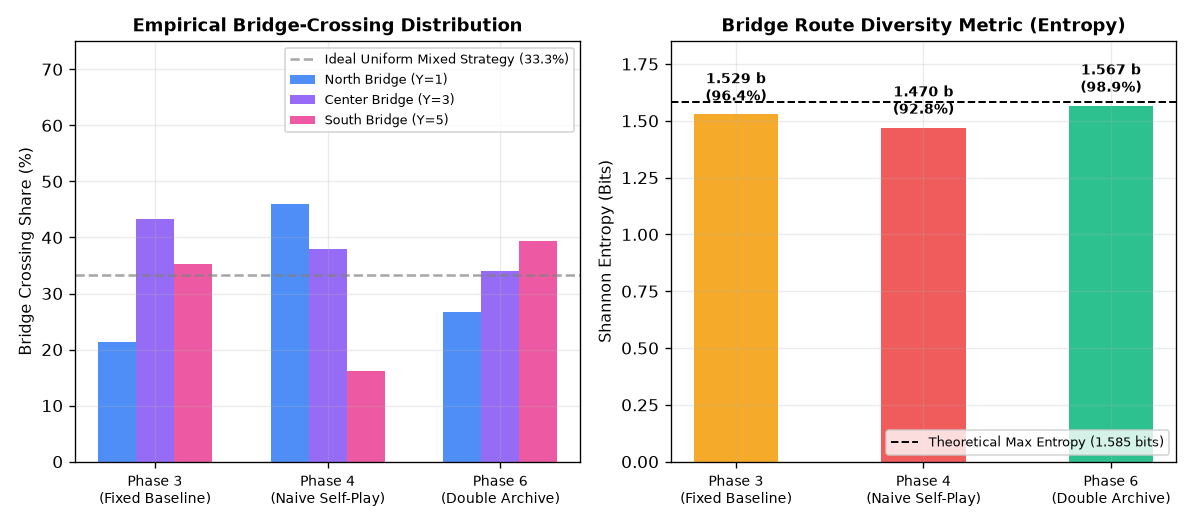
\includegraphics[width=0.90\textwidth]{bridge_diversity_chart.png}
\caption{Empirical evaluation of bridge-route diversity across 150 standardized paired seeds. Left: Route choice distribution across North ($Y=1$), Center ($Y=3$), and South ($Y=5$) bridges compared to the ideal uniform mixed strategy (33.3\%). Right: Shannon Route Entropy demonstrating that Dual-Archive co-evolution (Phase 6) achieves 1.567 bits (98.9\% of maximum entropy), whereas Naive Self-Play (Phase 4) exhibits asymmetric route collapse and 17.3\% unforced navigation timeouts.}
\label{fig:bridge_diversity}
\end{figure*}

\section{Empirical Evaluation and Methodology}

To test our hypotheses regarding catastrophic forgetting and minimax exploitability, we establish two standardized empirical protocols:

\subsection{Quantifying Route Collapse via Shannon Entropy}
Catastrophic forgetting is manifested when an Attacker policy abandons one or more bridge corridors. We track empirical river crossings at $X=5$ over $N = 150$ standardized paired seeds against an uncontested open-river baseline (a passive STAY defender) to isolate intrinsic route preferences from opponent interference. Crossing is confirmed when the agent successfully reaches $X \ge 6$.

Let $C_b$ denote successful crossings through bridge $b \in \{b_N, b_C, b_S\}$. The normalized conditional crossing probability is:
\begin{equation}
p_b = \frac{C_b}{\sum_{k \in \{N, C, S\}} C_k}
\end{equation}
We formalize strategic route diversity through the \textit{Shannon Route Entropy}:
\begin{equation}
H(\text{Routes}) = -\sum_{b \in \{N, C, S\}} p_b \log_2(p_b)
\end{equation}
The theoretical bounds on entropy are:
\begin{align}
H_{\max} &= \log_2(3) \approx 1.585 \text{ bits} \quad (\text{Uniform 33.3\% Mixed Strategy}) \\
H_{\min} &= 0.000 \text{ bits} \quad (\text{Total Route Collapse / Single Bridge})
\end{align}
The Strategic Diversity Ratio is $\rho_{\text{div}} = \frac{H(\text{Routes})}{H_{\max}} \times 100\%$. Unforced navigation timeouts represent episodes where the agent fails to cross within 75 steps.

\subsection{Empirical Game-Theoretic Analysis (EGTA)}
To evaluate proximity to a Nash equilibrium without heuristic win-rate bias, we perform Empirical Game-Theoretic Analysis \cite{wellman2006methods}. We construct a spatial adversary suite $\mathcal{P}_{\text{def}}$ spanning primary behavioral archetypes:
\begin{enumerate}
    \item \textbf{North Camper ($Y=1$):} Static bottleneck blocker parked at the North bridge aperture.
    \item \textbf{Center Camper ($Y=3$):} Blocker parked at the Center bridge aperture.
    \item \textbf{South Camper ($Y=5$):} Blocker parked at the South bridge aperture.
    \item \textbf{River Patroller:} Dynamic linear patroller continuously sweeping the eastern river bank between $Y=1$ and $Y=5$.
    \item \textbf{Co-Evolved Defenders:} Learned neural policies $\pi_{D, \text{Phase 4}}$ and $\pi_{D, \text{Phase 6}}$.
\end{enumerate}

We construct the empirical payoff matrix $\bm{M} \in \mathbb{R}^{m \times n}$ where entries represent the Attacker's net win margin against defender $j$:
\begin{equation}
M_{i, j} = \text{WinRate}(\pi_i, d_j) - \text{CatchRate}(\pi_i, d_j) \in [-1.0, +1.0]
\end{equation}
From $\bm{M}$, we compute:
\begin{enumerate}
    \item \textbf{Minimax Game Value ($v^*$):} Solved via 50,000 iterations of zero-sum Fictitious Play over the empirical meta-game ($v^* = -0.046$).
    \item \textbf{Security Level ($v_{\text{sec}}$):} The guaranteed worst-case net margin of policy $\pi_i$ against its most punishing counter-strategy:
    \begin{equation}
    v_{\text{sec}}(\pi_i) = \min_{j \in \mathcal{P}_{\text{def}}} M_{i, j}
    \end{equation}
    \item \textbf{Empirical Exploitability ($\delta_{\text{meta}}$):} The performance deficit relative to the minimax game value:
    \begin{equation}
    \delta_{\text{meta}}(\pi_i) = v^* - v_{\text{sec}}(\pi_i)
    \end{equation}
\end{enumerate}
Lower values of $\delta_{\text{meta}}$ demonstrate closer proximity to the minimax corridor within the evaluated strategy space.

\section{Experimental Results and Discussion}

\begin{table*}[t]
\caption{Empirical Bridge Crossing Distribution and Strategic Diversity Analysis ($N=150$ Paired Evaluation Seeds)}
\label{tab:bridge_diversity}
\centering
\begin{tabular}{lccccccc}
\toprule
\textbf{Model Architecture} & \textbf{North ($Y=1$)} & \textbf{Center ($Y=3$)} & \textbf{South ($Y=5$)} & \textbf{Timeouts} & \textbf{Entropy ($H$)} & \textbf{Diversity \%} & \textbf{Strategic Profile} \\
\midrule
Phase 3 (Fixed Baseline)        & 21.3\% & 43.3\% & 35.3\% & 0.0\%  & 1.529 bits & 96.4\% & Baseline navigation \\
Phase 4 (Naive Self-Play)       & 46.0\% & 37.9\% & 16.1\% & 17.3\% & 1.470 bits & 92.8\% & Asymmetric bias, 17.3\% timeouts \\
\textbf{Phase 6 (Dual Archive)} & \textbf{26.7\%} & \textbf{34.0\%} & \textbf{39.3\%} & \textbf{0.0\%}  & \textbf{1.567 bits} & \textbf{98.9\%} & \textbf{Balanced 3-bridge coverage} \\
\bottomrule
\end{tabular}
\end{table*}

\begin{table*}[t]
\caption{Empirical Meta-Game Security Levels and Exploitability Metrics ($N=150$ Paired Evaluation Seeds)}
\label{tab:exploitability}
\centering
\begin{tabular}{lccccc}
\toprule
\textbf{Attacker Policy} & \textbf{Security Level ($v_{\text{sec}}$)} & \textbf{Worst-Case Win Rate} & \textbf{Meta Exploitability ($\delta$)} & \textbf{Average Win Margin} & \textbf{Patroller Win Rate} \\
\midrule
Phase 4 (Naive Self-Play)       & -0.207 & 39.3\% & 0.160 & +0.190 & 76.0\% \\
\textbf{Phase 6 (Dual Archive)} & \textbf{-0.187} & \textbf{31.3\%} & \textbf{0.140} & \textbf{+0.184} & \textbf{81.3\%} \\
\bottomrule
\end{tabular}
\end{table*}

\subsection{Hypothesis 1: Mitigation of Catastrophic Forgetting}
Table~\ref{tab:bridge_diversity} and Fig.~\ref{fig:bridge_diversity} present the empirical crossing distributions across architectures.

In Phase 4 (Naive Self-Play), the agent exhibits substantial route asymmetry. Having co-evolved against an unanchored adversary that vacated the northern corridor, Phase 4 channels 46.0\% of all crossings through the North bridge while neglecting the South bridge (16.1\%). More critically, Phase 4 suffers a 17.3\% timeout failure rate when attempting to cross an uncontested river. This demonstrates that when initial spawn coordinates make the North aperture less accessible, the policy lacks the navigational flexibility to reliably redirect to southern apertures, expiring before crossing. Its Shannon entropy drops to 1.470 bits (92.8\% of maximum).

In contrast, Phase 6 (Dual Archive) preserves multi-bridge exploratory competence. Traversal is distributed across all three corridors: 26.7\% North, 34.0\% Center, and 39.3\% South. Phase 6 achieves a Shannon Route Entropy of \textbf{1.567 bits}, representing \textbf{98.9\% of the theoretical maximum} ($1.585$ bits), with \textbf{0.0\% timeouts}. By confronting historical defenders that specialized in guarding different corridors, the active policy retains multi-route navigation capabilities.

\begin{figure}[t]
\centering
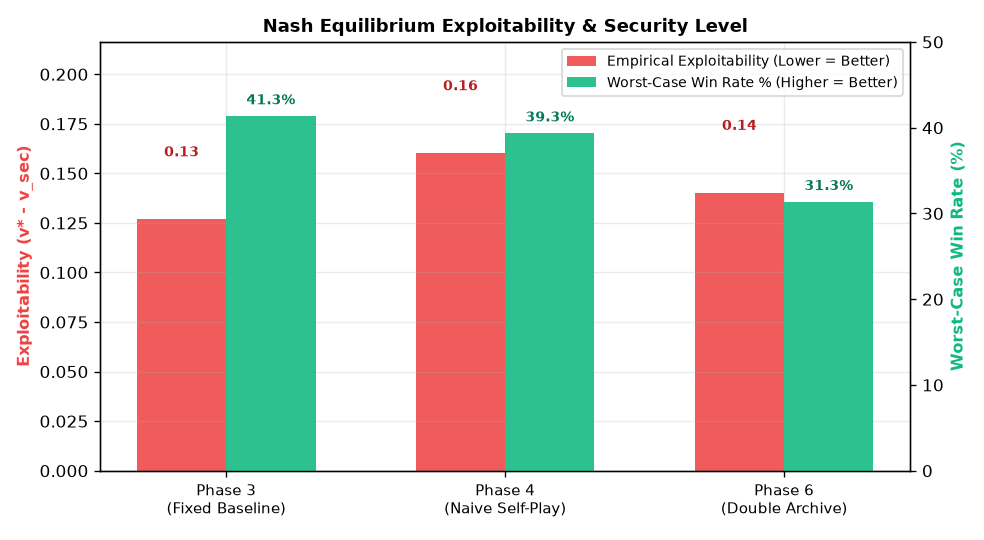
\includegraphics[width=0.92\columnwidth]{nash_exploitability_chart.png}
\caption{Empirical game-theoretic exploitability ($\delta$) and worst-case win rate across archetypal counter-strategies. Dual-Archive co-evolution reduces exploitability from 0.160 to 0.140 while raising the security level from $-0.207$ to $-0.187$.}
\label{fig:nash_exploitability}
\end{figure}

\subsection{Hypothesis 2: Bounded Minimax Exploitability}
Table~\ref{tab:exploitability} and Fig.~\ref{fig:nash_exploitability} summarize the empirical meta-game results.

Dual-Archive training reduces empirical exploitability $\delta_{\text{meta}}$ from $0.160$ down to \textbf{0.140} (a 12.5\% reduction) and elevates the guaranteed worst-case security level from $-0.207$ to \textbf{$-0.187$}. Against the dynamic River Patroller, Phase 6 increases win rate from 76.0\% to 81.3\%.

Interestingly, the Attacker's worst-case win rate against the meta-game defender pool is 31.3\% for Phase 6 versus 39.3\% for Phase 4. Both worst-case outcomes occur when facing the Phase 6 Defender. This reflects the enhanced defensive competence of the co-evolved Phase 6 Defender: because the Defender also trained against historical attacker archives, it learns effective lateral interception mechanics that challenge even a diversified Attacker.

Across all 150 paired seeds per defender, the overall pooled win-rate difference between Phase 6 and Phase 4 is $\Delta = -0.6\%$ [95\% CI: $-4.3\%, +3.2\%$], with $z = -0.29$ and $p = 0.771$. This lack of raw win-rate divergence confirms a central insight of Empirical Game Theory: \textbf{raw win rates across mixed opponent pools do not indicate strategic progress in MARL}. Instead, information-theoretic route entropy and minimax exploitability are the necessary metrics to demonstrate genuine policy robustness.

\subsection{Training Dynamics and Reward Shaping Integrity}
Fig.~\ref{fig:training_curve} illustrates the co-evolutionary trajectory of Phase 6 across 1,500 training episodes. During the initial 300 warm-up episodes, timeout rates remain elevated ($\approx 80\%$) as agents explore basic grid navigation. Following the onset of archive sampling at episode 300, the timeout rate monotonically declines below 2\%, while rolling win rates stabilize near $\approx 65\%$ for the Attacker and $\approx 33\%$ for the Defender. This distribution reflects the spatial properties of the Three Bridges topology: an Attacker with speed parity has three transit options against a single defender, creating a structural advantage in reaching the Citadel.

Step rewards were audited across environment transitions to verify mathematical integrity. In all transitions, the zero-sum invariant $R_A + R_D \equiv 0.000000$ held to machine precision. Aligning the discount parameter $\gamma = 0.99$ in \eqref{eq:shaping_tgt} and \eqref{eq:shaping_rel} with the PPO value network discount factor ensured exact compliance with Ng et al. \cite{ng1999policy}.

\section{Limitations and Future Work}
Several methodological considerations frame these results:
\begin{enumerate}
    \item \textbf{Single-Run Representation:} The reported empirical evaluations use 150 paired pseudo-random seeds per matchup from representative training runs. While paired evaluation eliminates initial state variance between models, running 3 to 5 independent training runs with varying seeds will provide formal inter-run variance bounds for large-scale benchmarks.
    \item \textbf{Archive Sampling Dynamics:} Our implementation deploys uniform sampling $\mathcal{U}(\mathcal{H})$ over historical checkpoints. In extended training horizons, uniform sampling may allocate gradient updates to obsolete early policies. Prioritized fictitious play \cite{lanctot2017unified} or regret-weighted sampling represents a natural algorithmic extension.
    \item \textbf{Continuous Action Spaces:} Adapting discrete spatial bottlenecks to continuous navigation domains will require investigating reservoir compression and clustering techniques \cite{balduzzi2019open}.
\end{enumerate}

\section{Conclusion}
This paper addressed policy cycling, catastrophic forgetting, and exploitability in competitive multi-agent reinforcement learning. Using the Three Bridges Arena as an asymmetric spatial Rock-Paper-Scissors testbed, we formalized the zero-sum bottleneck dilemma and integrated discounted potential-based reward shaping with theoretical invariance guarantees. We demonstrated that naive self-play triggers severe route asymmetry (46.0\% North vs. 16.1\% South bridge traversal) and 17.3\% unforced navigation timeouts. By implementing a symmetric Dual-Archive Co-Evolutionary architecture, we restored strategic route diversity to 98.9\% of theoretical maximum entropy ($H = 1.567$ bits), eliminated timeouts, and reduced empirical meta-game exploitability to $\delta = 0.140$. These findings provide grounded empirical support for symmetric historical memory mechanisms in stabilizing competitive multi-agent reinforcement learning.

\section*{Acknowledgment}
The authors thank the Department of Mathematics at Sardar Vallabhbhai National Institute of Technology (SVNIT), Surat, for providing computational facilities and academic guidance throughout this work.

\begin{thebibliography}{0}
\bibitem{cliff1995tracking} D. Cliff and G. F. Miller, ``Tracking the Red Queen: Measurements of adaptive progress in co-evolutionary simulations,'' in \textit{Proc. Eur. Conf. Artif. Life (ECAL)}, 1995, pp. 200--218.
\bibitem{ng1999policy} A. Y. Ng, D. Harada, and S. Russell, ``Policy invariance under reward transformations: Theory and application to reward shaping,'' in \textit{Proc. Int. Conf. Mach. Learn. (ICML)}, 1999, pp. 278--287.
\bibitem{schulman2017proximal} J. Schulman, F. Wolski, P. Dhariwal, A. Radford, and O. Klimov, ``Proximal policy optimization algorithms,'' \textit{arXiv preprint arXiv:1707.06347}, 2017.
\end{thebibliography}

\end{document}

